\begin{figure}[h!]
    \begin{center}
        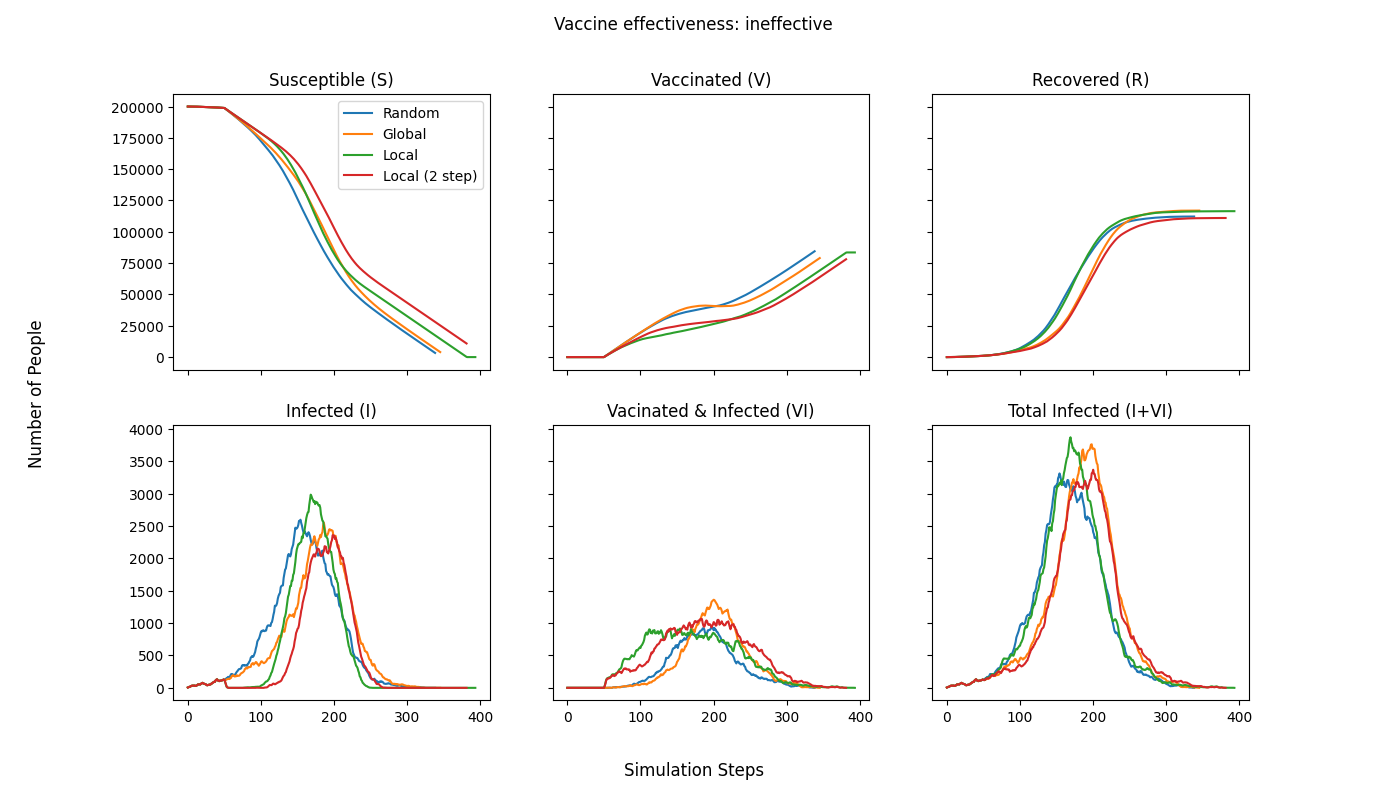
\includegraphics[width=1\textwidth]{Q6-none.png}
        \caption{Figure showing the how changing the vaccination strategy effects the course of an outbreak. Red - random strategy. Yellow - globally target nodes of highest degree. Green - target nodes of highest degree on infection fringe. Local (2 step) - an extension of the local strategy that targets nodes most at risk 2 steps in the future.} 
        \label{fig:q6-none}
    \end{center}
\end{figure}

\begin{figure}[h!]
    \begin{center}
        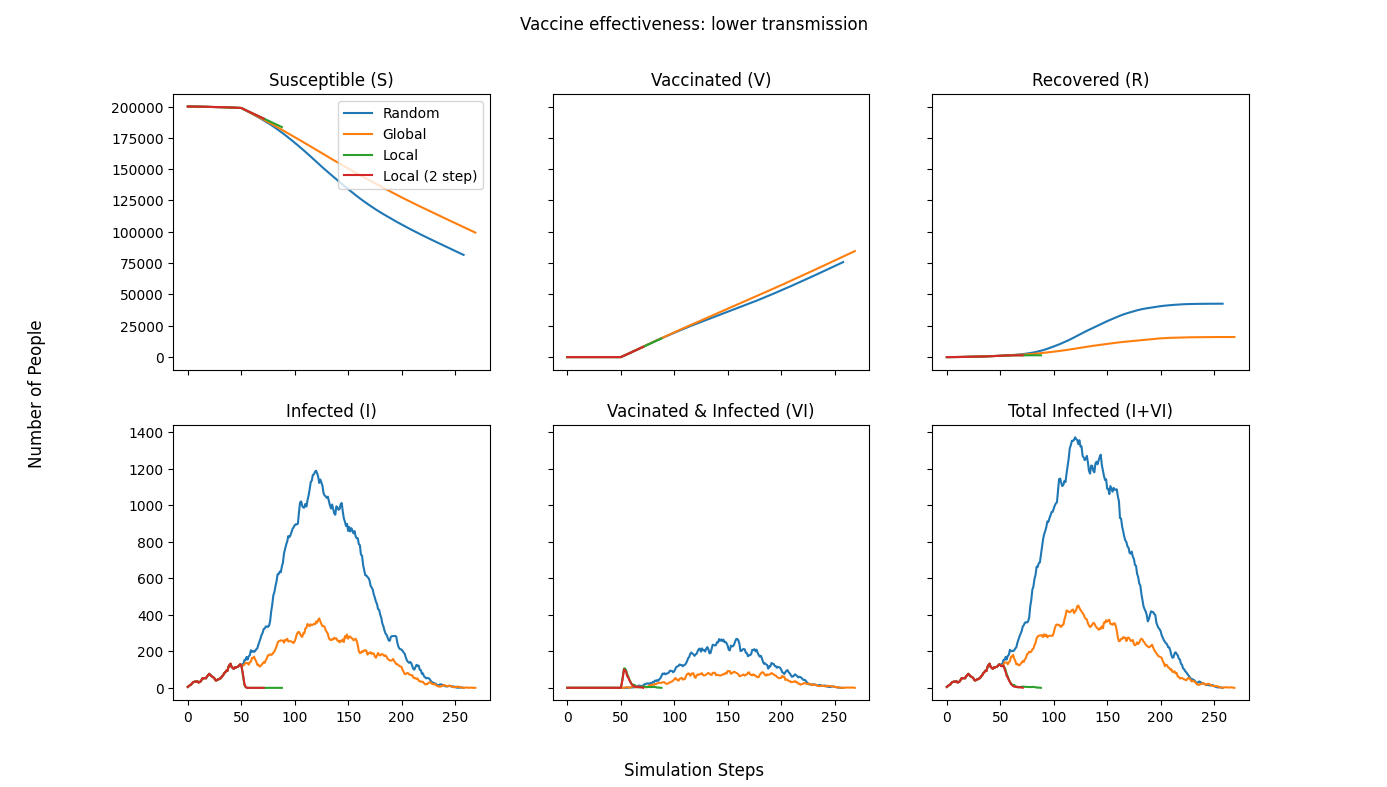
\includegraphics[width=1\textwidth]{Q6-transmit.png}
        \caption{Figure showing the how changing the vaccination strategy effects the course of an outbreak. Red - random strategy. Yellow - globally target nodes of highest degree. Green - target nodes of highest degree on infection fringe. Local (2 step) - an extension of the local strategy that targets nodes most at risk 2 steps in the future.} 
        \label{fig:q6-transmit}
    \end{center}
\end{figure}

\begin{figure}[h!]
    \begin{center}
        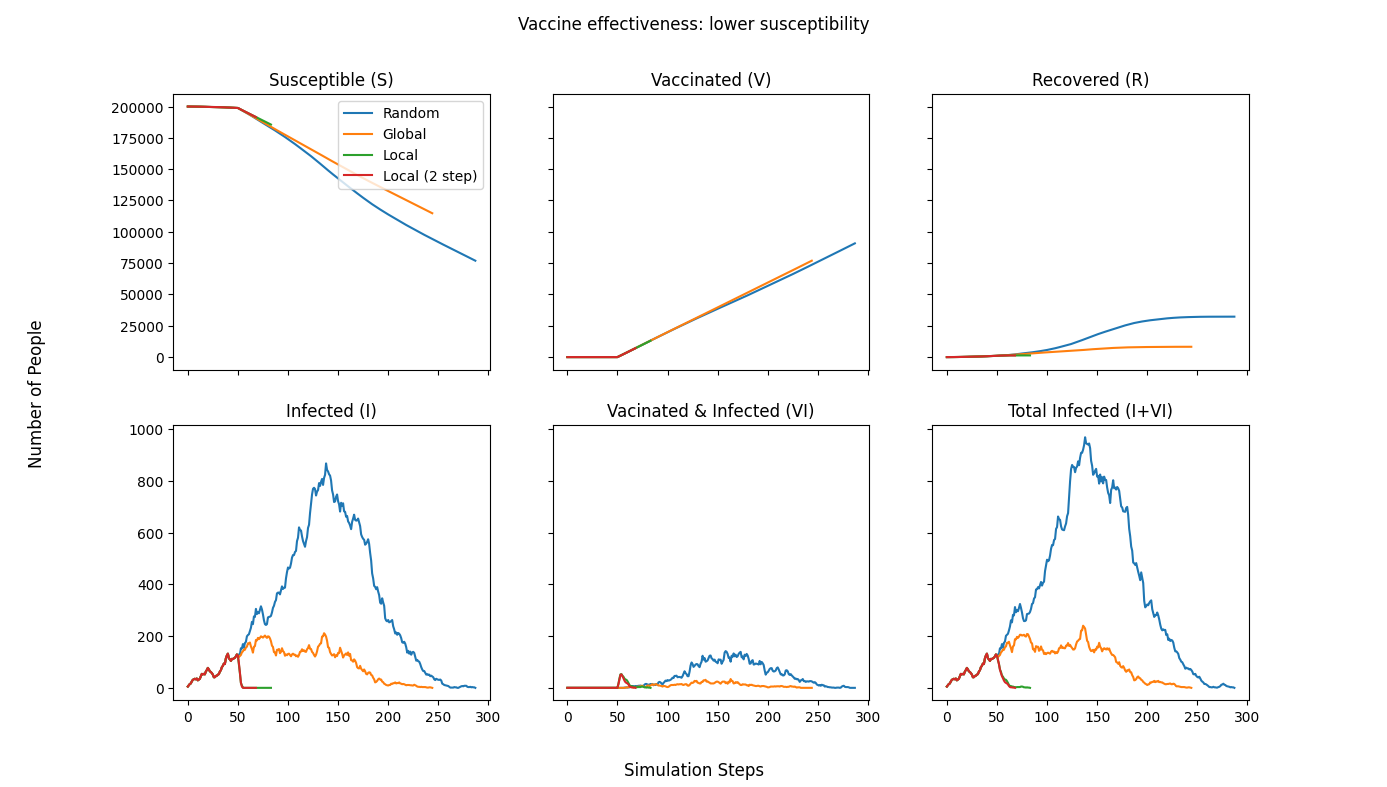
\includegraphics[width=1\textwidth]{Q6-catch.png}
        \caption{Figure showing the how changing the vaccination strategy effects the course of an outbreak. Red - random strategy. Yellow - globally target nodes of highest degree. Green - target nodes of highest degree on infection fringe. Local (2 step) - an extension of the local strategy that targets nodes most at risk 2 steps in the future.} 
        \label{fig:q6-catch}
    \end{center}
\end{figure}

\begin{figure}[h!]
    \begin{center}
        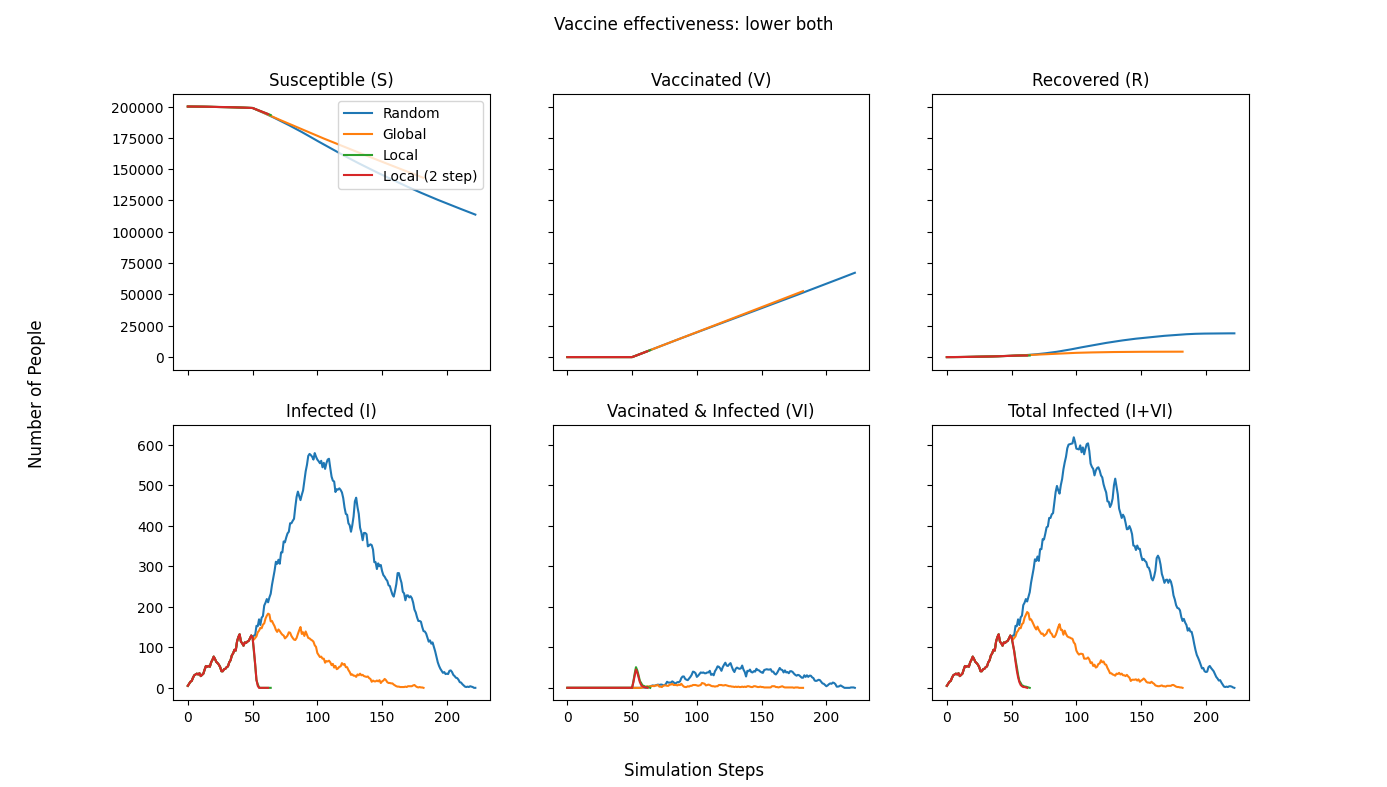
\includegraphics[width=1\textwidth]{Q6-both.png}
        \caption{Figure showing the how changing the vaccination strategy effects the course of an outbreak. Red - random strategy. Yellow - globally target nodes of highest degree. Green - target nodes of highest degree on infection fringe. Local (2 step) - an extension of the local strategy that targets nodes most at risk 2 steps in the future.} 
        \label{fig:q6-both}
    \end{center}
\end{figure}